% This is a basic Math Paper

\documentclass[11pt]{article}

% Preamble

\usepackage[margin=1in]{geometry}
\usepackage{amsfonts, amsmath, amssymb}
\usepackage{fancyhdr, float, graphicx}
\usepackage[utf8]{inputenc} % Required for inputting international characters
\usepackage[T1]{fontenc} % Output font encoding for international characters
\usepackage{fouriernc} % Use the New Century Schoolbook font
\usepackage[nottoc, notlot, notlof]{tocbibind}
\usepackage{url}
\usepackage[font=itshape]{quoting}

% Header and Footer
\pagestyle{fancy}
\fancyhead{}
\fancyfoot{}
\fancyhead[L]{\textit{\Large{Film Review of Invictus}}}
%\fancyhead[R]{\textit{something}}
\fancyfoot[C]{\thepage}
\renewcommand{\footrulewidth}{1pt}



% Other Doc Editing
% \parindent 0ex
%\renewcommand{\baselinestretch}{1.5}

\begin{document}
	
	\begin{titlepage} 
		\centering 
		
		%---------------------------NAMES-------------------------------
		
		\huge\textsc{
			MIT World Peace University
		}\\
	
		\vspace{0.75\baselineskip} % space after Uni Name
		
		\LARGE{
			Human Dynamics and Peace and Communications\\
			First Year B. Tech, Trimester 3\\
			Academic Year 2021-22
		}
		
		\vfill % space after Sub Name
		
		%--------------------------TITLE-------------------------------
		
		\rule{\textwidth}{1.6pt}\vspace*{-\baselineskip}\vspace*{2pt}
		\rule{\textwidth}{0.6pt}
		\vspace{0.75\baselineskip} % Whitespace above the title
		
		
		
		\huge{\textsc{
				Film Appreciation of Invictus
			}} \\
		
		
		
		\vspace{0.5\baselineskip} % Whitespace below the title
		\rule{\textwidth}{0.6pt}\vspace*{-\baselineskip}\vspace*{2.8pt}
		\rule{\textwidth}{1.6pt}
		
		\vspace{1\baselineskip} % Whitespace after the title block

		%--------------------------SUBTITLE --------------------------	
			
		\LARGE\textsc{
			Assignment 3
		} % Subtitle or further description
		\vfill
		
		%--------------------------AUTHOR-------------------------------
		
		Prepared By
		\vspace{0.5\baselineskip} % Whitespace before the editors
		
		\Large{
			109054. Krishnaraj Thadesar
						
			Division 9 Batch I3
		}
		
		
		\vspace{0.5\baselineskip} % Whitespace below the editor list
		\today

	\end{titlepage}

\tableofcontents
\clearpage
	

\section{Outline of the Story}

\noindent
\begin{minipage}{0.6\textwidth}\raggedright
\textbf{Invictus} is a 2009 biographical sports drama film
directed by Clint Eastwood and starring Morgan
Freeman and Matt Damon. The story is based on
the 2008 John Carlin book \textit{Playing the Enemy:
	Nelson Mandela} and the Game That Made a
Nation about the events in South Africa before
and during the 1995 Rugby World Cup.
The story portrays the struggles faced by South
Africa post Apartheid, and how their new
President – Nelson Mandela adapted to these new
changes and helped in uniting the Nation once and
for all.\\
\underline{\textbf{Rugby}} was a nationally loved sport and in a
way, the heart of South Africa. Mandela saw
Rugby as an opportunity to revive the spirit of
the New and United South Africa.
The Film very accurately and thoroughly
portrays how he does this with the help of the
South African Captain - \textit{François Pienaar}.\\
\vspace{5mm}
\end{minipage}
\hfill%
\begin{minipage}{0.3\textwidth}% adapt widths of minipages to your needs
	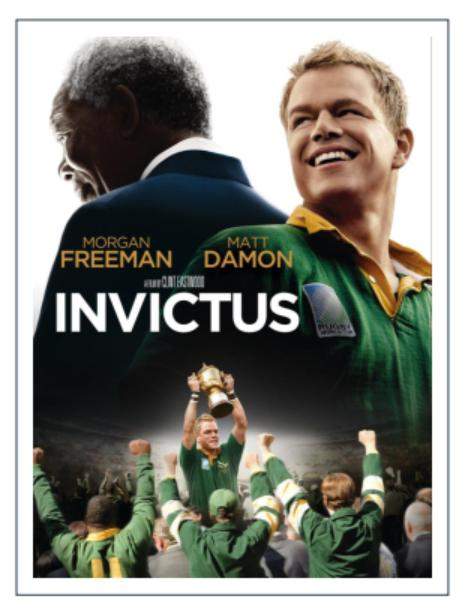
\includegraphics[width=\linewidth]{cover.jpg}
\end{minipage}\\

It also shows how the people of South Africa
reacted to the new changes.
The differences between them diminished
eventually, but the tension after and before
the election saw a lot of discrimination, racism
and panic. That is also accurately and
sensitively represented in the film.
\section{Central Theme}
\textit{Newly elected President Mandela} knows his nation remains racially and
economically divided in the wake of apartheid. Believing he can bring his
people together through the universal language of sport, Mandela rallies
South Africa's underdog rugby team as they make an unlikely run to the
1995 World Cup Championship match.\\

\textbf{Leadership} forms a major theme of the film. In meeting with Francois,
Mandela asks him how a leader can inspire those he leads to greatness,
to be better than they think they can be. Leaders appeal to “the better
angels of our nature,” encouraging the best in us and more both by their
actions and example.
\section{Key Moments}
Throughout the film, there were several Key
moments that were major turning points
and had they been done any differently,
they would have changed the course of
history as we know it now. Some of them are shown below. 

\subsection{Nelson Mandela Takes Oath as the President of South Africa}

\begin{figure}[H]
	\centering
	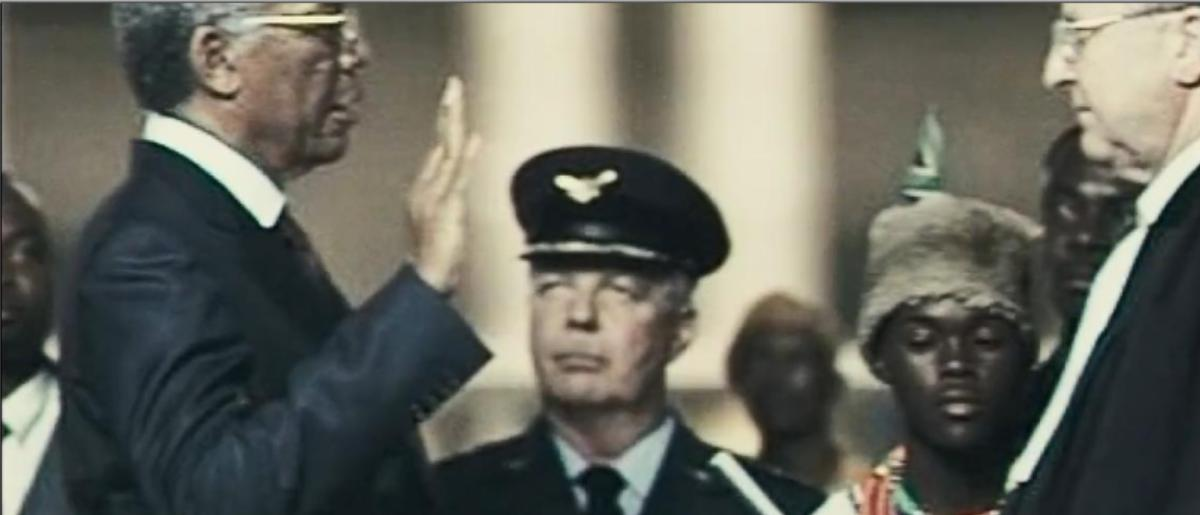
\includegraphics[scale=0.4]{1.jpg}
\end{figure}



\subsection{Captain Francois' Speech Inspires the Team before the Final}

\begin{figure}[H]
	\centering
	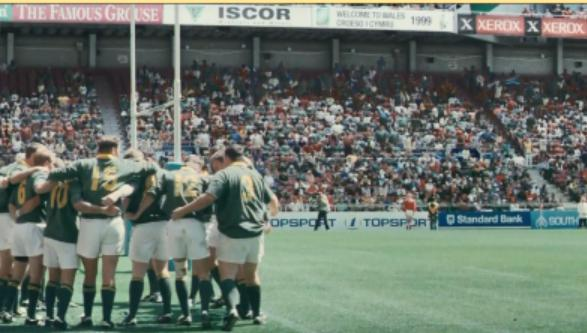
\includegraphics[scale=0.8]{2.jpg}
\end{figure}

\subsection{President Mandela Meets Captain Francois}


\begin{figure}[H]
	\centering
	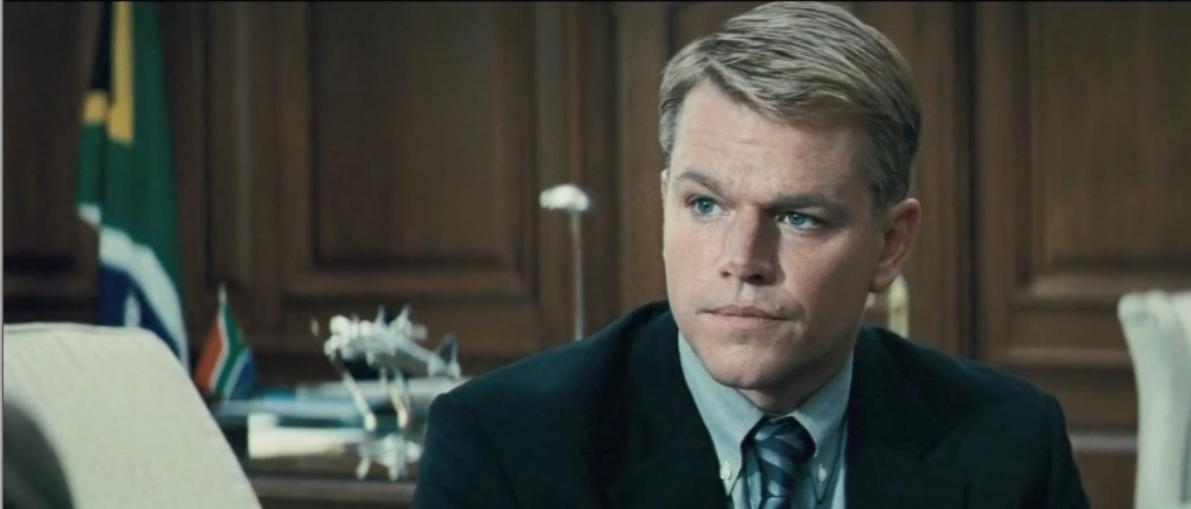
\includegraphics[scale=0.4]{3.jpg}
	\caption{President Mandela Invites Captain Francois}
\end{figure}

\begin{figure}[H]
	\centering
	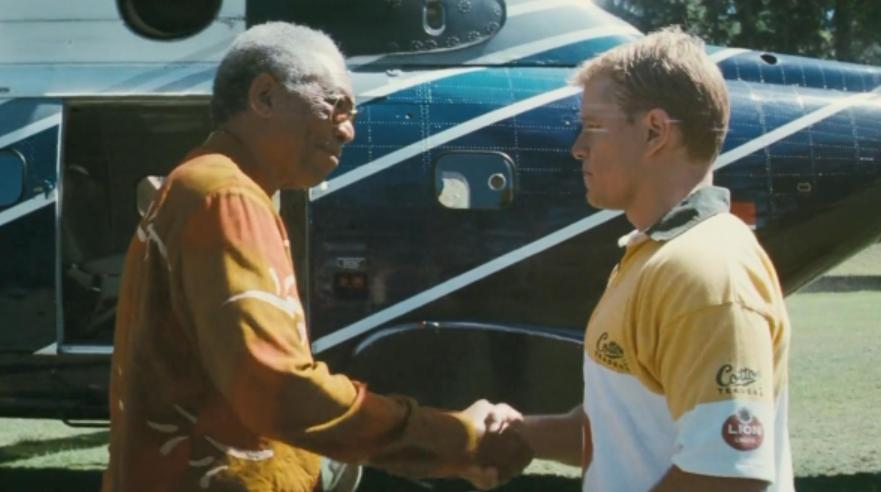
\includegraphics[scale=0.5]{3.1.jpg}
	\caption{President Mandela Meets Francois to wish him luck before the game}
\end{figure}


\subsection{The President's Security Guards Celebrate Together}

\begin{figure}[H]
	\centering
	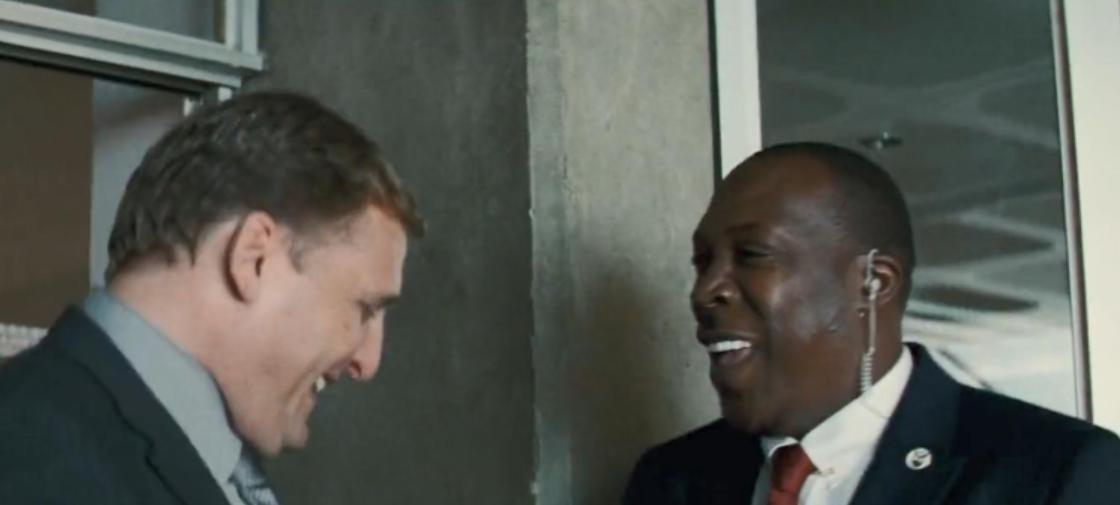
\includegraphics[scale=0.4]{4.jpg}
	\caption{Guards put aside their racial differences and celebrate in unity}
\end{figure}

\subsection{White Policemen Celebrate with a Local Kid}

\begin{figure}[H]
	\centering
	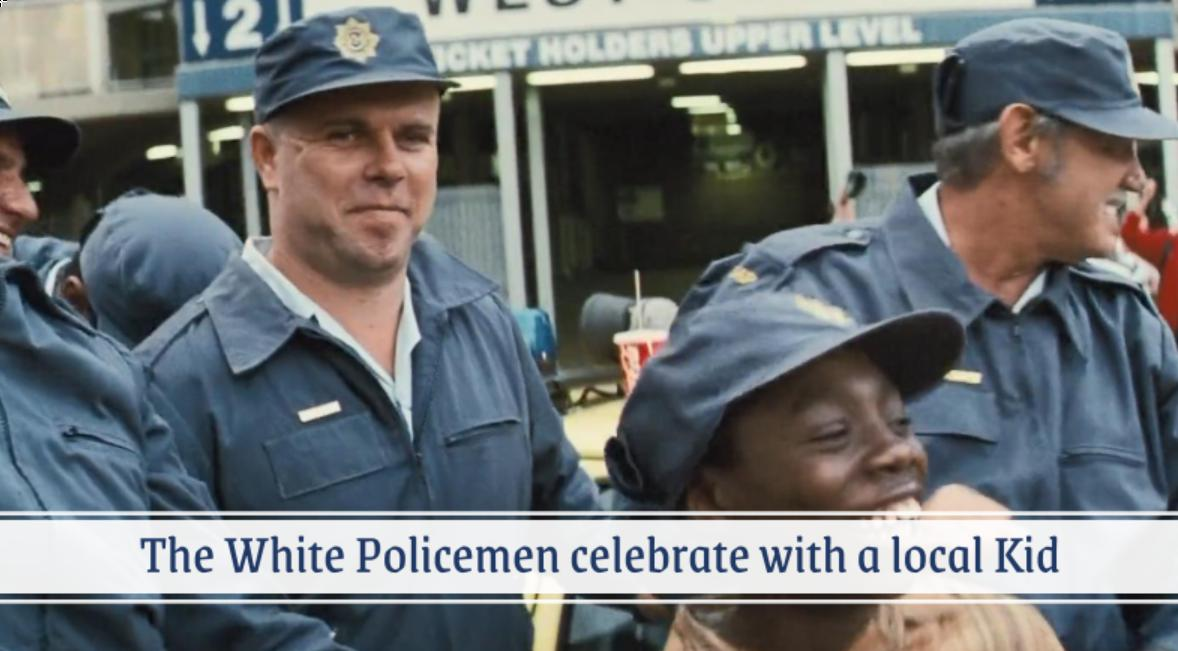
\includegraphics[scale=0.37]{5.jpg}
\end{figure}

\section{Critical Views}
The film was very well reviewed and well critiqued. It had aimed to portray the
struggles of Mandela in uniting a broken and deeply wounded South Africa post
Apartheid – and it accomplishes that in excellent manner. A movie about Racial
Injustice, Discrimination, and Suffering is just as much about Leadership,
Inspiration and of the many other things – \textit{Rugby}.
It performed very well, and the credit must definitely go to the storyline, and
acting, and \textit{Morgan Freeman’s Mandela} single-handedly grabs your attention
throughout, while being equally complemented by \textit{Matt Damon’s Francois
Pienaar.}
It is so well played in fact, that when a shot of the real Mandela appears over the
final credits, it's momentarily jarring to realize you've been watching an
impersonation.
\section{What we can Learn}
The Movie Makes us realize countless things that often go
unnoticed. It teaches us everything from \textit{leadership} and
\textit{perseverance} to Rugby and \textit{Teamspirit}, and does it incredibly
well. Some of the things that were taught in the movie, through
the character and image of Mandela himself are shown below. 
\subsection{Passion Produces Perseverance}
Not only was the \textit{Madiba}
willing to unite South Africa,
he was passionate about his
dream of a country, one that
was united and treated
everyone equally. It didn’t
matter if he had to wait 27
years for it. It didn’t matter if
only the entire world ridiculed
him for it. All that mattered
was the passion that gave him
the energy to persevere
through everything that came
his way.
\subsection{Violence is not the Answer}
No matter how bad the
situations got in front of him, he
never even thought of
considering violence to combat
it. This is primarily because he
had faced and had been a victim
of it himself. He knew that there
was no end to it, and that if we
decided to follow this path, it
would only get dirtier and
bloodier along the way.
\subsection{Learn how to Forgive}
What the \textit{Madiba} achieved in his tenure is quite shocking, not just
because of what he did, but because of how he did it. The self control and
forgiveness that he showed to his people was phenomenal and
infectious. He led a group of people that he was a part of and convinced
them and himself that they were now a part of something bigger that
included their enemies. Even saying it out loud will cause confusion in
your head. Voluntarily putting back all the grudges of your past and
forgiving everyone who has ever done anything wrong to you and your
people is perhaps not even imaginable, and yet was achieved
spectacularly.
\subsection{How to Bond by sharing Experiences}
A political leader in his position could have either given speeches and
parades, a couple of paragraphs in the local Newspaper, and maybe a few
TV interviews in hopes of diffusing the situation, But Mandela firmly
believed that if you want to bond the country, words were clearly not
enough. You needed something to bond over, which in this case was the
National Sport Rugby. That Final Match is still believed to have been the
one that united a nation.\\

\begin{quotation}
	\textit{Sport has the power to change the world. It has the power to inspire, it has the power to unit people, and in a way that little else does}\\
	\begin{flushright}
		Nelson Mandela
	\end{flushright}
\end{quotation}


	
\end{document}